\subsection{Probability Based Tiling}
\label{sec:ProbTiling}
%\subsubsection*{Motivation}

The next algorithm we propose exploits the inherent biases among the leaves of a decision tree. In typical machine learning models some leafs (equivalently outcomes or predictions) are more likely to be reached than others. In such settings, having balanced tiled trees is not sufficient to minimize expected inference time. 

Consider for example two machine learning models \op{airline-ohe} and \op{epsilon} (also used in our evaluation). 
Consider the graphs shown in   
figures \ref{Fig:AirlineOHEStats} and \ref{Fig:EpsilonStats} that are generated from training data. Each line in these graphs corresponds to a fixed fraction of the input (say $f$). 
A point on a line at coordinate $(x, y)$ means that a fraction $y$ of trees in the model could cover a fraction $f$ of all training inputs with a fraction $x$ of 
leaves. For example, the first point on the $f=0.9$ line in figure \ref{Fig:AirlineOHEStats} says that about 52\% of trees ($y$ value) need only 1\% of their
leaves ($x$ value) to cover 90\% of the training input. 
In general, Figure \ref{Fig:AirlineOHEStats} shows that very few leaves are needed to cover a very large fraction of inputs for the benchmark \op{airline-ohe}. 
This means that a small fraction of leaves are very likely. 
We call trees with a small number of extremely likely leaves \textbf{\emph{leaf biased}}.

On the other hand, for the benchmark \op{epsilon},
figure \ref{Fig:EpsilonStats} shows that a trees need a much larger fraction of their leaves to cover a significant fraction of the training input.
This means that most trees in the \op{epsilon} model are not leaf biased.

\CommentOut{
\subsubsection{More Notation}
In order to formulate the probability based tiling algorithm as an optimization problem, we define the following.
\begin{enumerate}
    \item For every leaf $l \in L$, we define $p_l$ as the probability that the leaf $l$ is reached.
    \item For each node $n \in V$, we define the absolute probability $p_v$ as
    \begin{equation}
        p_v = \begin{cases}
        p_l &\text{if $l \in L$}\\
        p_{left(v)} + p_{right(v)} &\text{otherwise}
        \end{cases}
    \end{equation}
    \item For any tree $T$, $\mathcal{C}(T)$ represents the set of all valid tilings of $T$.
    \item For every $v \in V$, we define $S_v$ as the subtree rooted at $v$.
    \item For every $v \in V$, we define $L_v$ as the set of leaves of $S_v$.
    \item For a every tile $T_i$, we define $root(T_i)$ as the node $v \in T_i$ such that $v$ has no incoming edges from any other node $u \in T_i$.
    \item For a tile $T_i$, $out(T_i) \subseteq E$ is the set of edges $(u, v)$ such that $u \in T_i$ and $v \notin T_i$.
\end{enumerate}
}

\begin{figure}
    \centering
    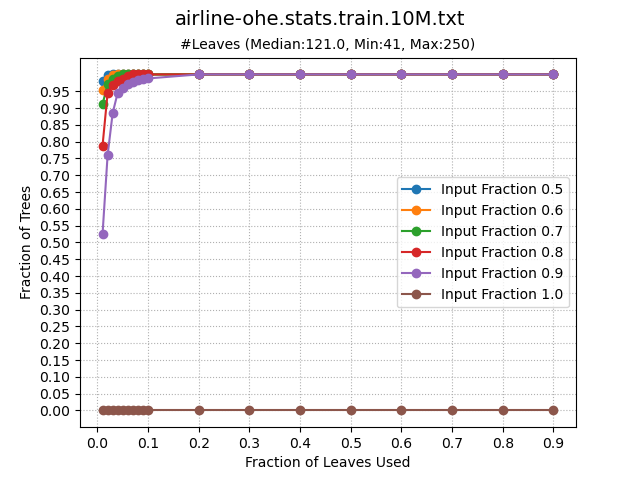
\includegraphics[width=\linewidth]{figures/airline-ohe.stats.train.txt.png}
    \caption{Statistical profile for airline-ohe}
    \label{Fig:AirlineOHEStats}
\end{figure}
\begin{figure}
    \centering
    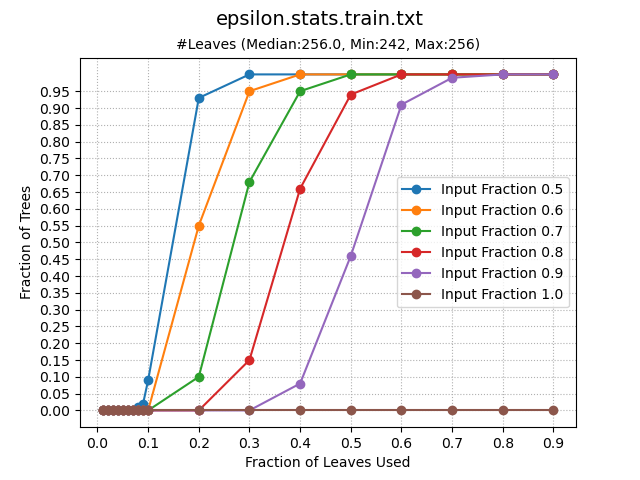
\includegraphics[width=\linewidth]{figures/epsilon.stats.train.txt.png}
    \caption{Statistical profile for epsilon}
    \label{Fig:EpsilonStats}
\end{figure}
\CommentOut{
We say that an input row $r_i$ is \textbf{\emph{covered}} by a subset of leaves $L' \subseteq L$ of a tree $T$, if the leaf $l$ reached by 
walking $T$ for row $r_i$ is in $L'$. We show how different models (and even different trees within the same model) behave differently 
using models for two benchmarks, airline-ohe and epsilon. Consider the graphs shown in   
figures \ref{Fig:AirlineOHEStats} and \ref{Fig:EpsilonStats}. Each line in these graphs corresponds to a fixed fraction of the input (say $f$). 
A point on a line at coordinate $(x, y)$ means that a fraction $y$ of trees in the model could cover a fraction $f$ of all training inputs with a fraction $x$ of 
leaves. For example, the first point on the $f=0.9$ line in figure \ref{Fig:AirlineOHEStats} says that about 52\% of trees ($y$ value) need only 1\% of their
leaves ($x$ value) to cover 90\% of the training input. 
In general, Figure \ref{Fig:AirlineOHEStats} shows that very few leaves are needed to cover a very large fraction of inputs for the benchmark airline-ohe. 
This means that a small fraction of leaves are very likely. On the other hand, for the benchmark epsilon,
figure \ref{Fig:EpsilonStats} shows that a trees need a much larger fraction of their leaves to cover a significant fraction of the test input.
This means that most trees in the epsilon model are not leaf biased.
One other observation we make is that most models have some leaf biased trees while the rest of the trees have equally likely leaves.
\TODO{AP Maybe define a term for trees with roughly equally likely leaves?} We design the probability based tiling algorithm to take advantage of this property 
of decision tree ensembles. 
}
\subsubsection{The Optimization Problem}

%We assume that we are given the probabilities of each leaf node of the decision tree (these can easily be computed using the training data). For every leaf $l \in L$, we %are given the probability $p_l$ that the leaf $l$ is reached. 

Observe that the latency of one tree walk is proportional to the number of tiles that need to be evaluated to reach the leaf. It is easy to see that for a leaf biased tree, basic tilling does not optimize for this objective, it considers all leafs to be equally likely. 
 
The goal of probablistic tiling is to minimize the average inference latency, or equivalently the minimize the expected number of tiles that are evaluated to compute one tree prediction. More formally, the problem is to find a \emph{valid} (as defined in Section~\ref{sec:ValidTiling}) tiling $\mathcal{T}$ such that the following objective is minimized.
\[
    \min_{\mathcal{T} \in \mathcal{C}(T)}{\sum_{l \in L} p_l.depth_{\mathcal{T}}(l)}
\]
where the minimization is over all valid tilings $\mathcal{T}$ of the tree $T$, $depth_{\mathcal{T}}(l)$ is the depth of the leaf $l$ given tiling ${\mathcal{T}}$. $p_l$ is the probability of of reaching leaf $l$ as observed during training.

The above optimization problem can be solved optimally using dynamic programming. 
We leave this out in the interest of space. 
Instead, we use the simple greedy algorithm listed in algorithm \ref{Alg:GreedyTilingAlgo} to construct a valid tiling given the node probabilities\footnote{Probabilites for internal nodes can be computed from probablities for leafs by summing up the probabilities of all leafs that belong to the sub-tree rooted at the internal node. Leaf probabilities are collected during training.}.
The algorithm starts at the root and greedily keeps adding the most probable legal node to the current tile until the maximum tile size is reached.
Subsequently, the tiling procedure is recursively performed on all nodes that are destinations for edges going out of the constructed tile.

% \subsubsection{Dynamic Programming Formulation}


% For any node $v \in V$, we define
% \[
%     cost(v, \mathcal{T}) = \sum_{l \in L_v} p(l | v).depth_{\mathcal{T}}(l)
% \]
% where $\mathcal{T} \in \mathcal{C}(T_v)$.

% Then, the objective function, for the tree $T_v$, can be rewritten as 
% \[
%     opt\_cost(v) = \min_{\mathcal{T} \in \mathcal{C}(T_v)}{cost(v, \mathcal{T})}
% \]

% The objective function can then be rewritten in the following recursive form.
% \[
%     opt\_cost(v) = \min_{T_0 \in TileShapes(n_t, v)}{1 + \sum_{(n_1, n_2) \in out(T_0)} p(n_1 | v)p(n_2 | n1)opt\_cost(n_2)}
% \]
% where $TileShapes(n_t, v)$ is the set of all tile shapes of size $n_t$ with root $v$. A straight forward substitution argument shows why the solution to the subproblems (tiling all sub-trees) needs to to be optimal. The objective is now in a form that can solved using
% dynamic programming. 

% \subsubsection{Greedy Algorithm}

% Intuitively, it seems like the following greedy algorithm also gives the optimal tiling. The algorithm starts at the root and greedily keeps adding the most probable node to the current tile until the maximum tile size is reached.
\begin{algorithm}
    \caption{Greedy Probability Based Tree Tiling}
    \label{Alg:GreedyTilingAlgo}
    \begin{algorithmic}
        \Procedure{TileTree}{$T = (V, E, r)$, $n_t$} 
            \If {$r \in L$}
                \State \textbf{return} $\{ r \}$
            \EndIf
            \State $Tile \leftarrow \{ r \}$
            \While{$|Tile| < n_t$}
                \State $e = (u,v) \in Out(Tile)$ st $p(v)$ is max and $v \notin L$
                \If{$e = \emptyset$}
                    \State \textbf{break}
                \EndIf
                \State $Tile = Tile \cup \{ v \}$
            \EndWhile
            \State $Tiles =  \{ Tile \}$
            \For{$(u,v) \in Out(Tile)$}
                \State $Tiles \leftarrow Tiles \cup TileTree(S_v, n_t)$
            \EndFor
            \State \textbf{return} $Tiles$
        \EndProcedure
    \end{algorithmic}
\end{algorithm}

% Talk about problems with increasing number of tile shapes and only performing such tiling on skewed trees
\CommentOut{
When we tried to apply algorithm \ref{Alg:GreedyTilingAlgo} on all trees in our benchmarks, we found
that even minor variations in probability caused the tiling algorithm to generate a large 
number of tile shapes. This in turn caused a loss in performance because the large size of the 
lookup table needed (section \ref{sec:LookupTable}) caused increased L1 cache misses. In order to 
alleviate this, we only perform probability based tiling on trees that are leaf biased.
}
We find probability based tiling is only beneficial for leaf biased trees\footnote{Turns out that probability based tiling produces many more tile shapes (see Section~\ref{sec:tileShapes}) which direclty impacts the cost of \op{getChildTile} making it more expensive than basic tiling}.  Recall that   
a tree to be leaf biased if a small fraction of leaves, say $\alpha$, can cover a large fraction of training inputs, say $\beta$.
We only perform probability based tiling on trees with thresholds $\alpha=0.05$ and $\beta=0.9$ and fall back to uniform tiling otherwise. 



